% Preamble
\documentclass{article}
\usepackage[left=1in, right=1in, top=1in, bottom=1in]{geometry}

% packages
\usepackage {lmodern}
\usepackage [T1]{fontenc}
\usepackage {amsmath}
\usepackage {amssymb}
\usepackage {amsfonts}
\usepackage {graphicx}
\usepackage {fullpage}
\usepackage {gensymb}
\usepackage {caption}
%\usepackage{nopageno}
\usepackage {cite}
\usepackage {setspace}
\usepackage [version=4]{mhchem}
\usepackage {multicol} 
\usepackage {sectsty}
\usepackage {textcomp}
\usepackage {pdfpages}

\newenvironment{nscenter}
    {\parskip=0pt\par\nopagebreak\centering}
    {\par\noindent\ignorespacesafterend}

% graphics path
\graphicspath {{images/}}

% bibliography style 
\bibliographystyle{unsrt}    

% font settings
	%%% headings font
	\sectionfont{\fontfamily{ptm}\fontsize{12}{15}\selectfont} 
	\subsectionfont{\fontfamily{ptm}\fontsize{10}{12}\selectfont}

	%%% paragraph font
	\usepackage{fontspec}
	\defaultfontfeatures{Mapping=tex-text, Scale=MatchLowercase}
	\setmainfont{Arial}

% Title
\title{Gas Chromatography - Mass Spectroscopy: \\
Determination of Caffeine in Coffee Using GC-MS}

\author{{Justin Chao*, Stephen Tung, and Luis Urbiola-Machado}\\[2ex]
The University of Texas at Austin \\ 
justin\_chao@utexas.edu \\ \\
November 29, 2016}
\date{}

% Begin Document
\begin{document}
\maketitle
\unskip\vspace{1.5\baselineskip}


\begin{multicols}{2}

{\fontsize{9.5}{12}\selectfont   

\section*{Abstract} 
The caffeine concentration of a coffee sample prepared under two different
    brewing conditions was determined using gas chromatography and mass
    spectrometry.
    The caffeine concentrations of Unknowns A and B were determined to be 768.1
    ppm and 1081 ppm respectively.
    As compared to literature, these results are determined to be slightly
    higher than expected values, due to human error in preparing the control
    sample.
    Furthermore, these findings are not precise do to the low number of trials.

\section*{Introduction}
This experiment aims to quantify the caffeine content of coffee under two
different brewing conditions using gas chromatography and mass spectroscopy. 
A sample of HEB brand Classic Roast, medium brewed
coffee was used in this experiment.

\subsection*{Gas Chromatography}
Gas Chromatography is a type of chromatography that is used to separate and
analyze components of a sample by vaporizing them. The mobile phase is
usually an inert carrier gas such as helium, and the stationary phase is
usually an inert liquid or polymer on the inside of the column. \cite{Harris}
Figure \ref{fig:gc} shows a diagram of a gas chromatograph.

\begin{nscenter}
    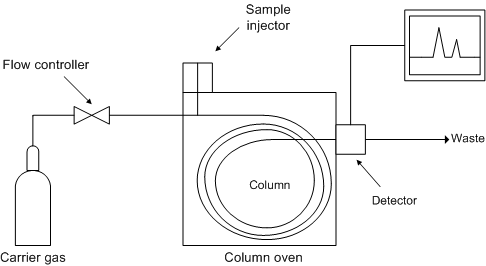
\includegraphics[scale=0.35]{gc.png}
    \captionof{figure}{Diagram of a gas chromatograph.\cite{gc_pic}}
    \label{fig:gc} 
\end{nscenter}

As the sample is injected into the column, the different components of the
sample are separated by their boiling points. Therefore, gas chromatography
is best suited for the analysis of more volatile compounds.

In this experiment a splitless injection is used, where an "on-instrument"
dilution is performed and the relative amounts of sample which enter the
column or is discarded to waste via the split line are adjusted using the
relative carrier and split flow rate ratio. \cite{injection} 
This method of injection is useful for performing trace analysis of samples.

\subsection*{Mass Spectrometry}
Mass spectrometry (MS) is an analytical technique that allows for the
identification and quantification of chemical species by ionizing the sample
and separating the ions by their mass-to-charge ratio. 
When a sample is ionized by electron bombardment, some of the molecules may
fragment into charged particles.
The charged particles can then be separated usually with the use of a magnetic or electric
field. \cite{ms_msu}

Figure \ref{fig:ms} provides a diagram of a mass spectrometer.

\begin{nscenter}
    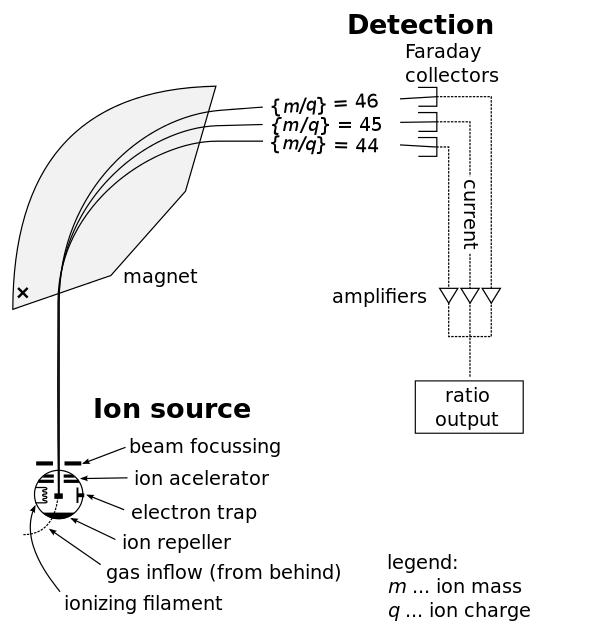
\includegraphics[scale=0.22]{ms.png}
    \captionof{figure}{Schematics of a simple mass spectrometer with sector type
    mass analyzer. This one is for the measurement of carbon dioxide isotope
    ratios (IRMS) as in the carbon-13 urea breath test. \cite{ms_wiki}}
    \label{fig:ms}
\end{nscenter}

There are two modes available for analyzing a sample through a mass
spectrometer: full scan and selected ion monitoring. Both methods have
their advantages as well as limitations. Please refer to the Discussion
portion of this report for further explanation.


\section*{Experimental}
\subsection*{Instrumental Parameters}
    A TRACE\texttrademark 1300, ITQ700 model Gas Chromatograph by Thermo-Fisher
    Scientific equipped with a Thermo-Finnigan POLARIS Ion Trap Mass
    Spectrometer was used in this experiment. 
    Table \ref{tab:param} provides the instrument parameters used in this
    experiment.

    \captionof{table}{Instrument parameters used in this experiment.}
    \begin{nscenter}
    \resizebox{0.45\textwidth}{!}{\begin{tabular}{l|c|l|c}
        \hline
        start time & 0.00 min. & scan mode & full scan \\
        ion polarity & positive & microscans & 3 \\
        max ion time & 25 ms & ion source temp. & 200$\degree$C \\

        initial oven temp & 40$\degree$C & hold time & 1 min. \\
        ramp rate & 0 & final oven temp. & 40$\degree$C \\
        hold time & n/a & EI voltage & 70 V \\

        inlet temp & 200$\degree$C & mode & split mode \\

        carrier pressure & 100.00 kPa & pressure mode & constant pressure \\
        MS transfer line temp & 50$\degree$C &  \\
        \hline
    \end{tabular}}
    \label{tab:param}
    \end{nscenter}

\subsection*{Sample Preparation}
Solutions of 250, 175, 100, and 25 ppm were prepared in 10 mL volumes
from a 1108.8 ppm stock solution to generate a calibration curve of caffeine
concentration. 
An amount of 4 mL of ethyl acetate was added to 1 mL of the unknown coffee
sample, and the solution was sonicated and centrifuged to separate the organic 
and aqueous layers.  
An amount of 0.1 g of anhydrous magnesium sulfate was then added to 1 mL of the
organic layer, and the mixture was agitated with a vortex mixer.  An amount of
50 μL of a $^{13}$C caffeine solution was then added to 250 μL of the organic
solution. 
Finally 1 μL of the prepared solution was injected into the gas chromatograph
for analysis. Each sample was run twice.

A control sample of 100.6 ppm caffeine in water was analyzed as well.
\cite{lab_man}

\section*{Results}
According to the Mayo Clinic, a brewed 8 oz cup of coffee may contain 95-200 mg
of caffeine.
The results of this experiment are deemed relatively accurate as compared to
literature values \cite{mayo}, but imprecise due to the low number of sample
trial runs. The reproducibility of these results is also unknown due to the lack
of sufficient number of sample runs.

Figure \ref{fig:cali_curve} shows the calibration curve generated from diluted
solutions of known caffeine concentrations.
\begin{center}
    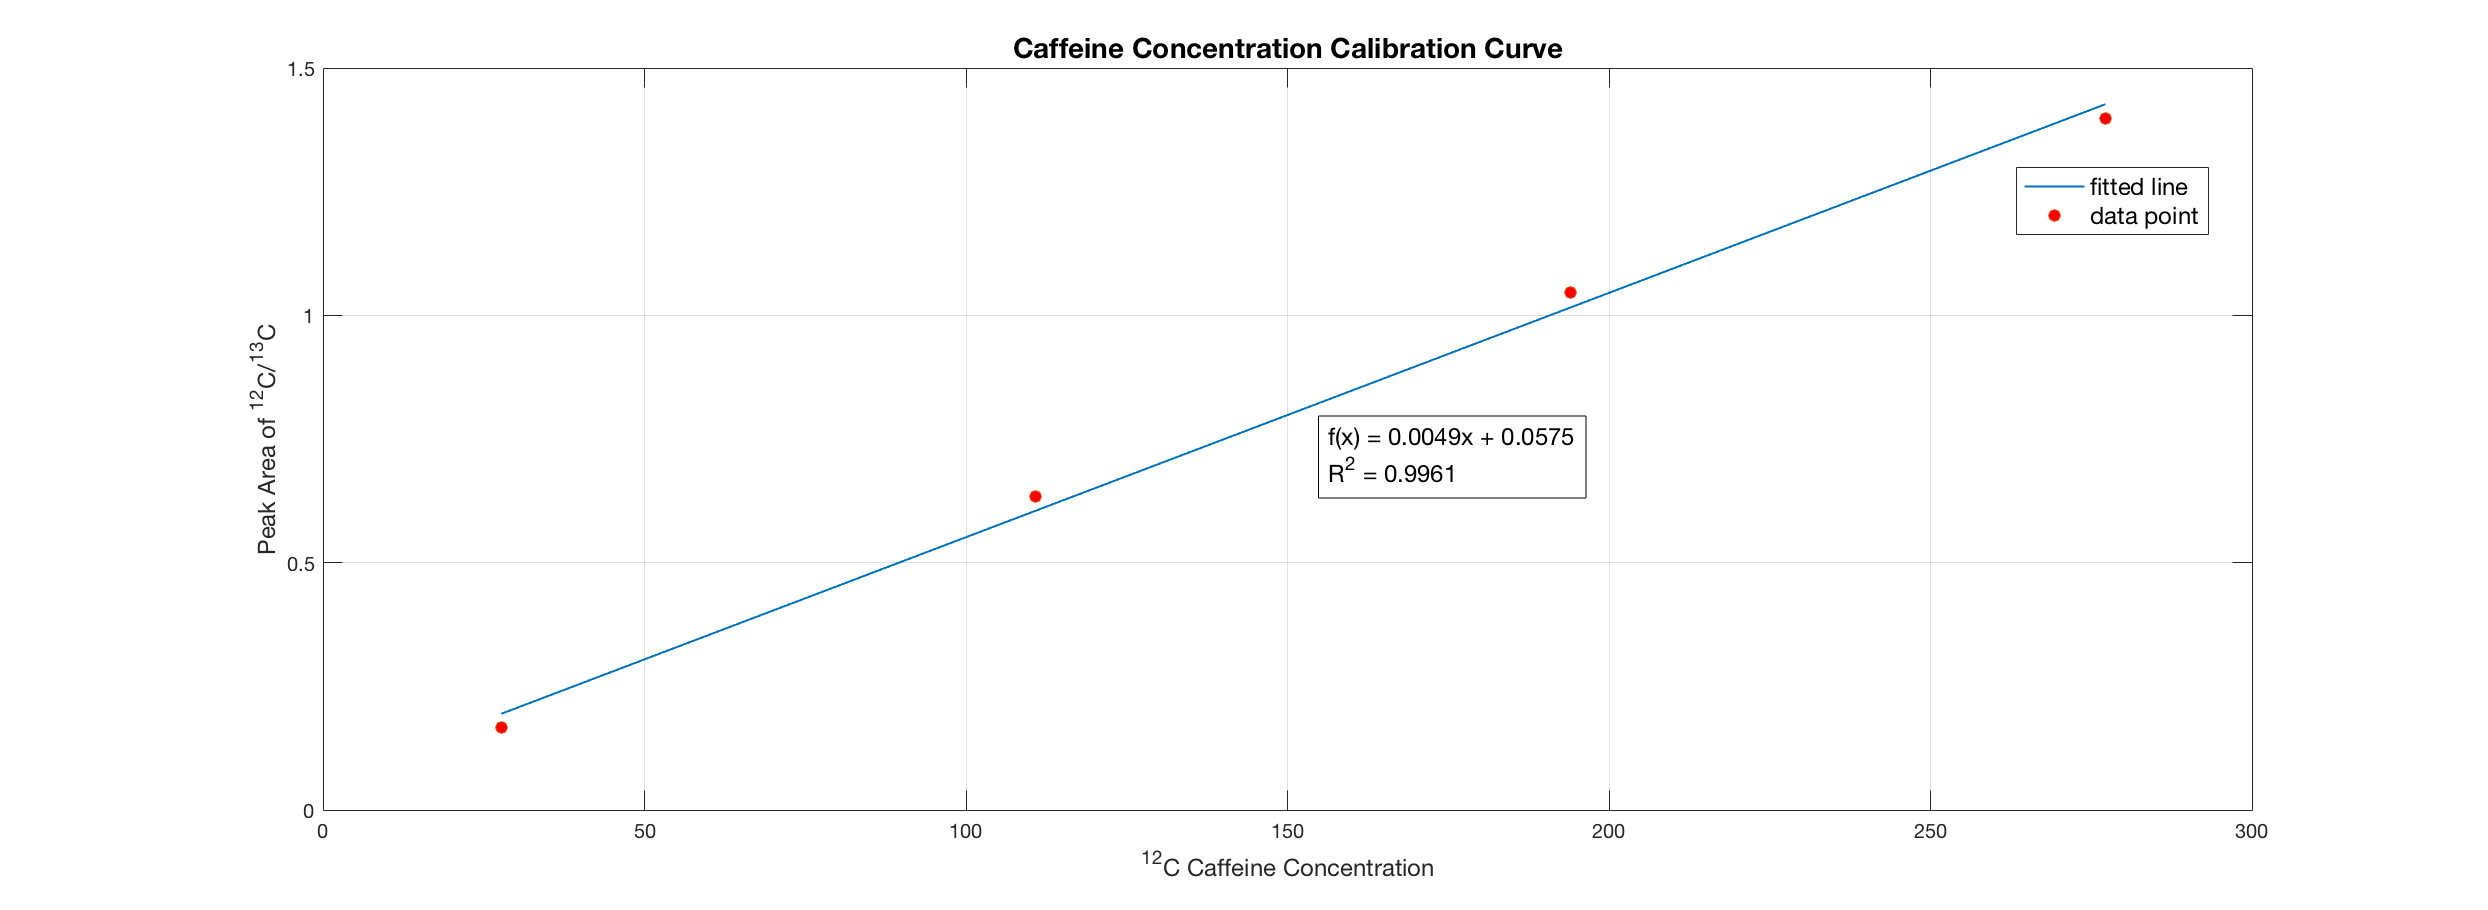
\includegraphics[scale=0.1]{calibration_curve}
    \captionof{figure}{Calibration curve of caffeine concentration.}
    \label{fig:cali_curve}
\end{center}

Tables \ref{tab:data} and \ref{tab:data2} lists the experimentally determined
caffeine concentrations of the unknown samples. 

\captionof{table}{Experimental results of caffeine concentration of unknowns.}
\begin{center}
\resizebox{0.4\textwidth}{!}{\begin{tabular}{c|c|c|c|c}
    & $^{12}$C caffeine conc. & Std dev. & RSD & 95\% CI \\
    \hline
    Unknown A & 768.1 ppm & 47.72 & 6.213 & 428.9 \\
    Unknown B & 1081 ppm & 99.54 & 9.205 & 894.6 \\
\end{tabular}}
\label{tab:data}
\end{center}

\captionof{table}{Experimental results of $^{12}$C caffeine concentrations in
unknowns.}
\begin{center}
\resizebox{0.3\textwidth}{!}{\begin{tabular}{c|c|c}
    & mg / fl oz & mg / 8 fl oz \\
    \hline
    Unknown A & 22.71 & 181.7 \\
    Unknown B & 31.98 & 255.8 \\
\end{tabular}}
    \label{tab:data2}
\end{center}

\section*{Discussion}
The results obtained in this experiment are slightly higher than expected
values. \cite{mayo} This is due to the control sample being prepared and run
with a different solution and parameters. Due to a loss of the original control
sample chromatogram data file, a separate data file from a different run was
used in calculating the extraction efficiency of the quantitative runs.
Calculations resulting from this control sample data returned a percent recovery of
128.4\%, which cannot be accurate.

Precision and reproducibility may also be improved with the inclusion of more trials.


[1] An internal standard is added in constant volumes to prepared sample
solutions. This is done so that a calibration curve may be constructed with the
ratio of the analyte signal to the signal of the internal standard, as a
function of the analyte concentration in the standard solutions. With this
technique, any loss of analyte during the preparation of the samples may be
corrected.

[2] When relatively large amounts of solvent are introduced during injection, a
solvent delay is set as a parameter for the mass spectrometer to turn off the
ionization source while the overloaded solvent peak elutes from the column. In
this experiment, a solvent delay is set to prevent rapid degradation of the
electron impact filament through rapid cooling by solvent vapor. Additionally,
large amounts of solvent ions may damage the interior of the MS.

[3] There are two modes available for analyzing a sample through a mass
spectrometer: full scan and selected ion monitoring (SIM). 
Full scan allows for the detection of multiple mass fragments across a
user-specified range. This method is useful for determining unknown compounds in
a sample. A total ion chromatogram is generated as well as a full mass spectrum,
which shows the intensity vs. ion mass of eluting ion masses at all times. This
mass spectrum can then be compared to literature for identifying compounds and
further sample analysis. If a large scan range is specified however, the
sensitivity of the instrument is decreased.
Selected ion monitoring only detects specific masses as defined by the user.
This level of specificity reduces background noise in a chromatogram and
improves detection sensitivity for the compound being analyzed. Disadvantages of
this method of course, include the need to know which masses to look for.

[4] A flame ionization detector (FID) detects ions formed during the combustion
of organic compounds, which limits this detection method to hydrocarbons.  On
the contrary, a mass spectrometer (MS) is able to detect a wide range of
compounds using their mass-to-charge ratio.  FIDs are relatively inexpensive to
operate and acquire, require little maintenance, and have fairly high linearity
and detection ranges for organic compounds. 
Mass spectrometers however, can be expensive and are easily prone to fouling.
Therefore if the compound of interest is organic, FIDs are a good choice for
analysis. Any other compounds, such as inorganic substances, would require the
use of an MS for analysis.

[5] According to the Mayo Clinic, a brewed 8 oz cup of coffee may contain
anywhere between 95 to 200 mg of caffeine. \cite{mayo}
In this experiment, caffeine concentrations for Unknowns A and B were determined
to be 181.7 and 255.8 mg / 8 fl oz. 
The wide range of values in literature may be a result of different brewing and
coffee oil extraction processes. Deviations of experimentally determined values
from literature values may be attributed to gross and human error, as the
control sample was run with different calibration and solution parameters.


\subsection*{Literature Review}
A refereed article that uses gas chromatography with mass spectrometry is the
article on "Methods of analysis by the U.S. Geological Survey National Water
Quality Laboratory; determination of pesticides in water by C-18 solid-phase
extraction and capillary-column gas chromatography/mass spectrometry with
selected-ion monitoring". \cite{article} 

In this article, the oven temperature was held at 100$\degree$C for 5 minutes,
then incremented at 6$\degree$C/min to 300$\degree$C, where it was then held for
5 minutes. A splitless injection method was used, and the mass spectrometer was
used with selected ion monitoring.


\section*{Conclusion}
The caffeine concentrations of Unknowns A and B were determined to be 768.1 ppm
and 1081 ppm respectively. As compared to literature \cite{mayo}, these
results are determined to be slightly higher than expected values (95-200 mg).

Sources of error may include random error on the part of the preparation of the
samples, as multiple people were involved in the process. Systematic error in
the handling of the GC/MS instrument and injection of samples may have also been
a factor.

The most probable cause of error however, is human error in the loss of the
original control sample chromatogram data file. Due to this error, an
alternative chromatogram of a control sample run in a previous experiment was
used resulting in an unreasonable percent recovery/extraction efficiency value
of 128.4\% for this data set.


\bibliography{GC-MS.bib}

}
\end{multicols}

\newpage
\section*{Appendix}
\begin{enumerate}
    \item Calibration curve of caffeine concentration.
    \item Chromatograms of calibration samples (25, 100, 175, 250 ppm).
    \item Chromatogram of Coffee Control Sample.
    \item Chromatograms of Coffee Sample A.
    \item Chromatograms of Coffee Sample B.
    \item Suggested pathway of fragmentation of caffeine.
    \item Sample calculations for determining caffeine concentration in Unknown
        A.
    \item Laboratory notebook copies with raw data.
\end{enumerate}

\newpage
\begin{center}
    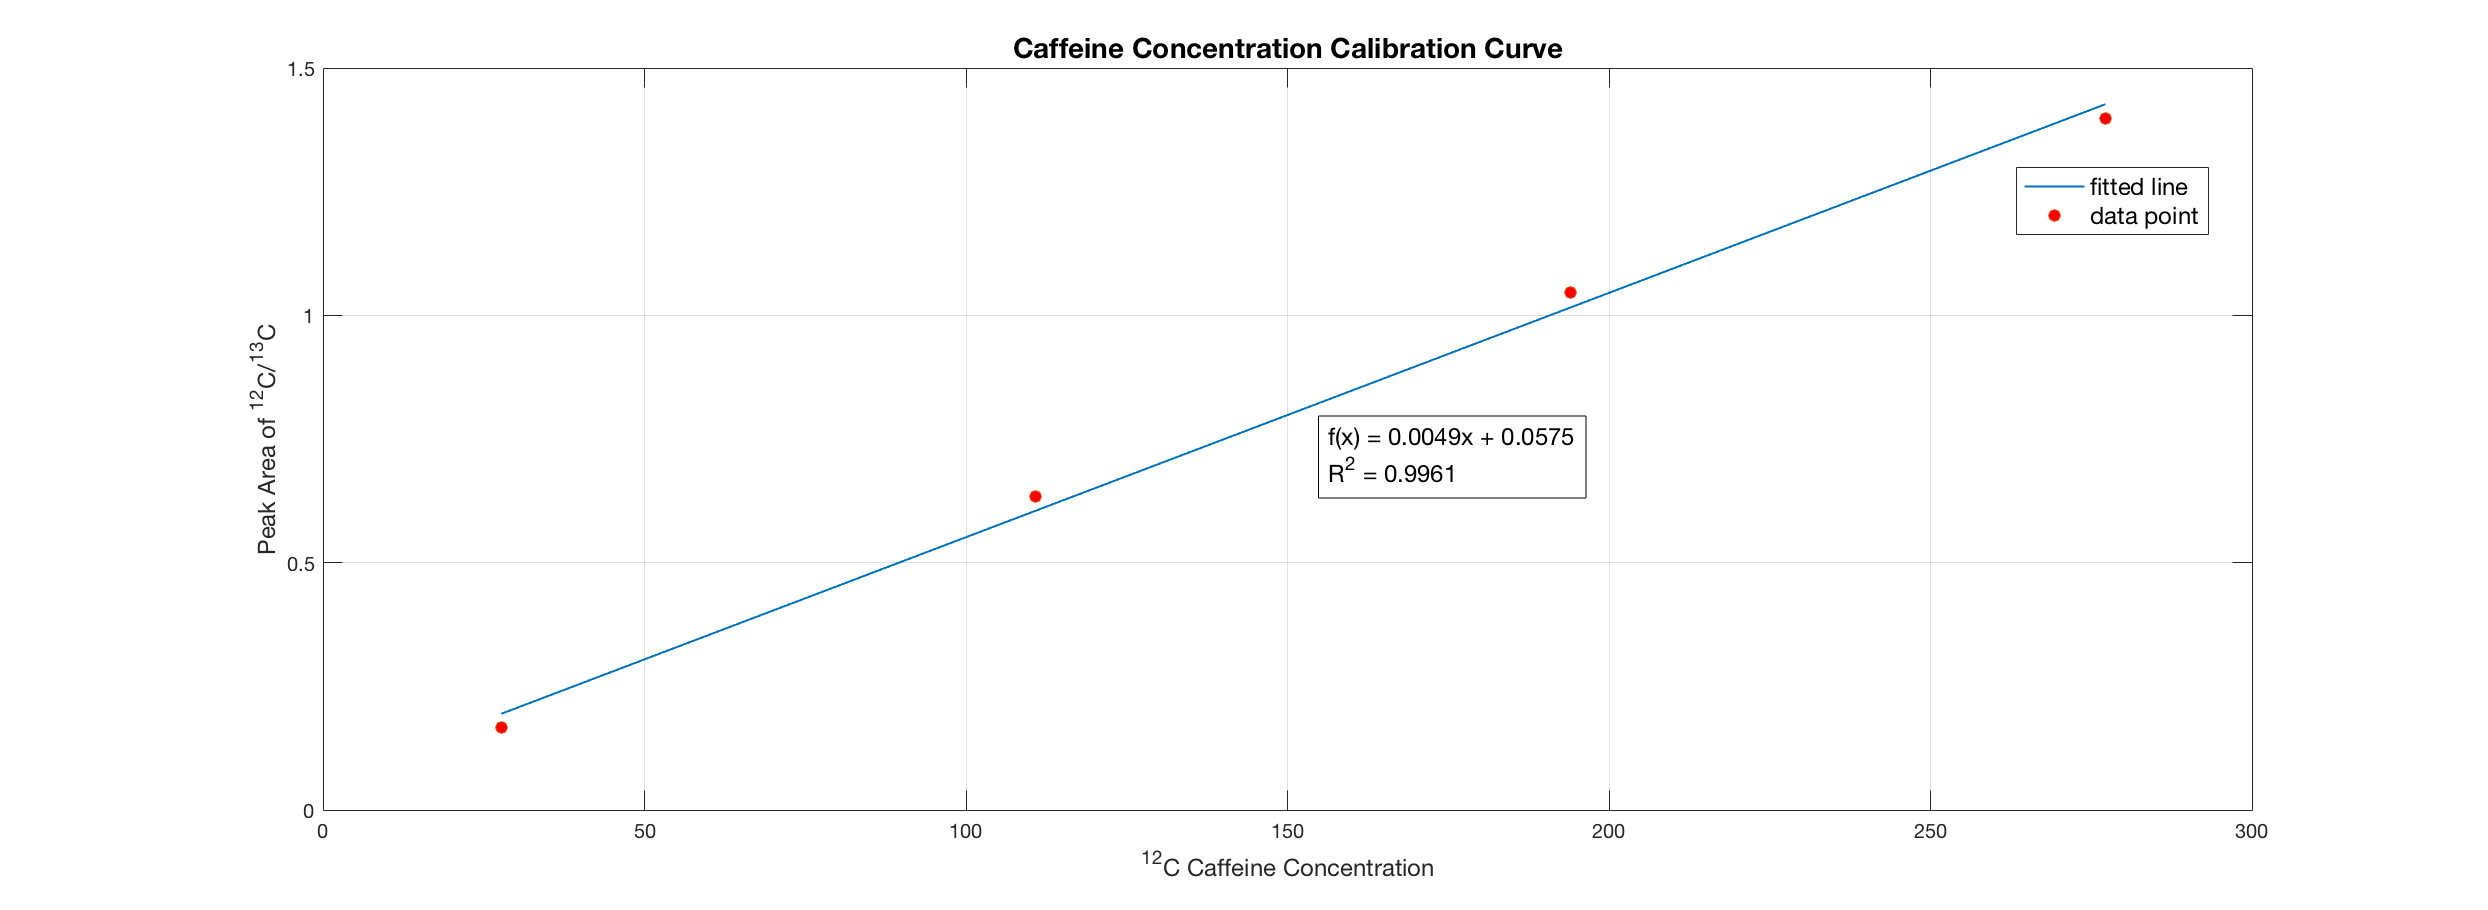
\includegraphics[scale=0.2]{calibration_curve}
    \captionof{figure}{Calibration curve of caffeine concentration.}
\end{center}

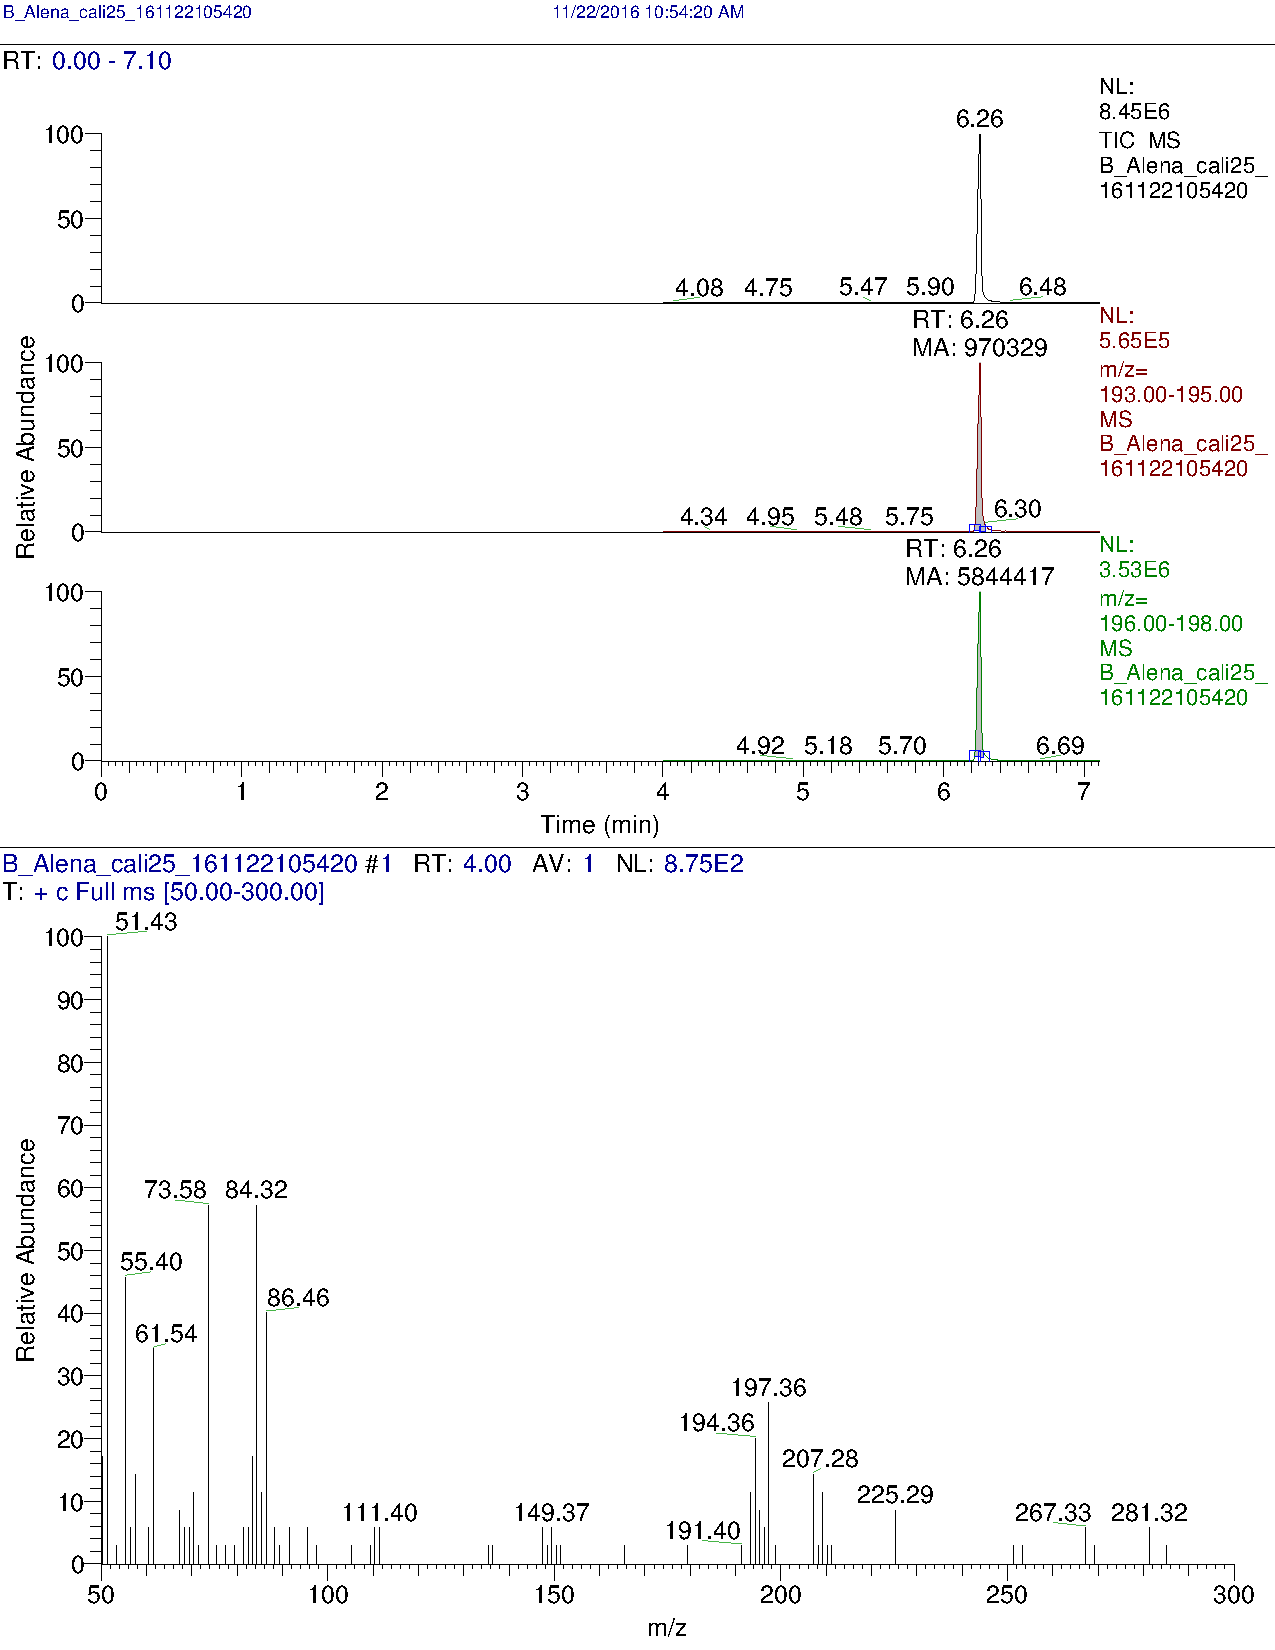
\includepdf[pages=-]{cali25.pdf}
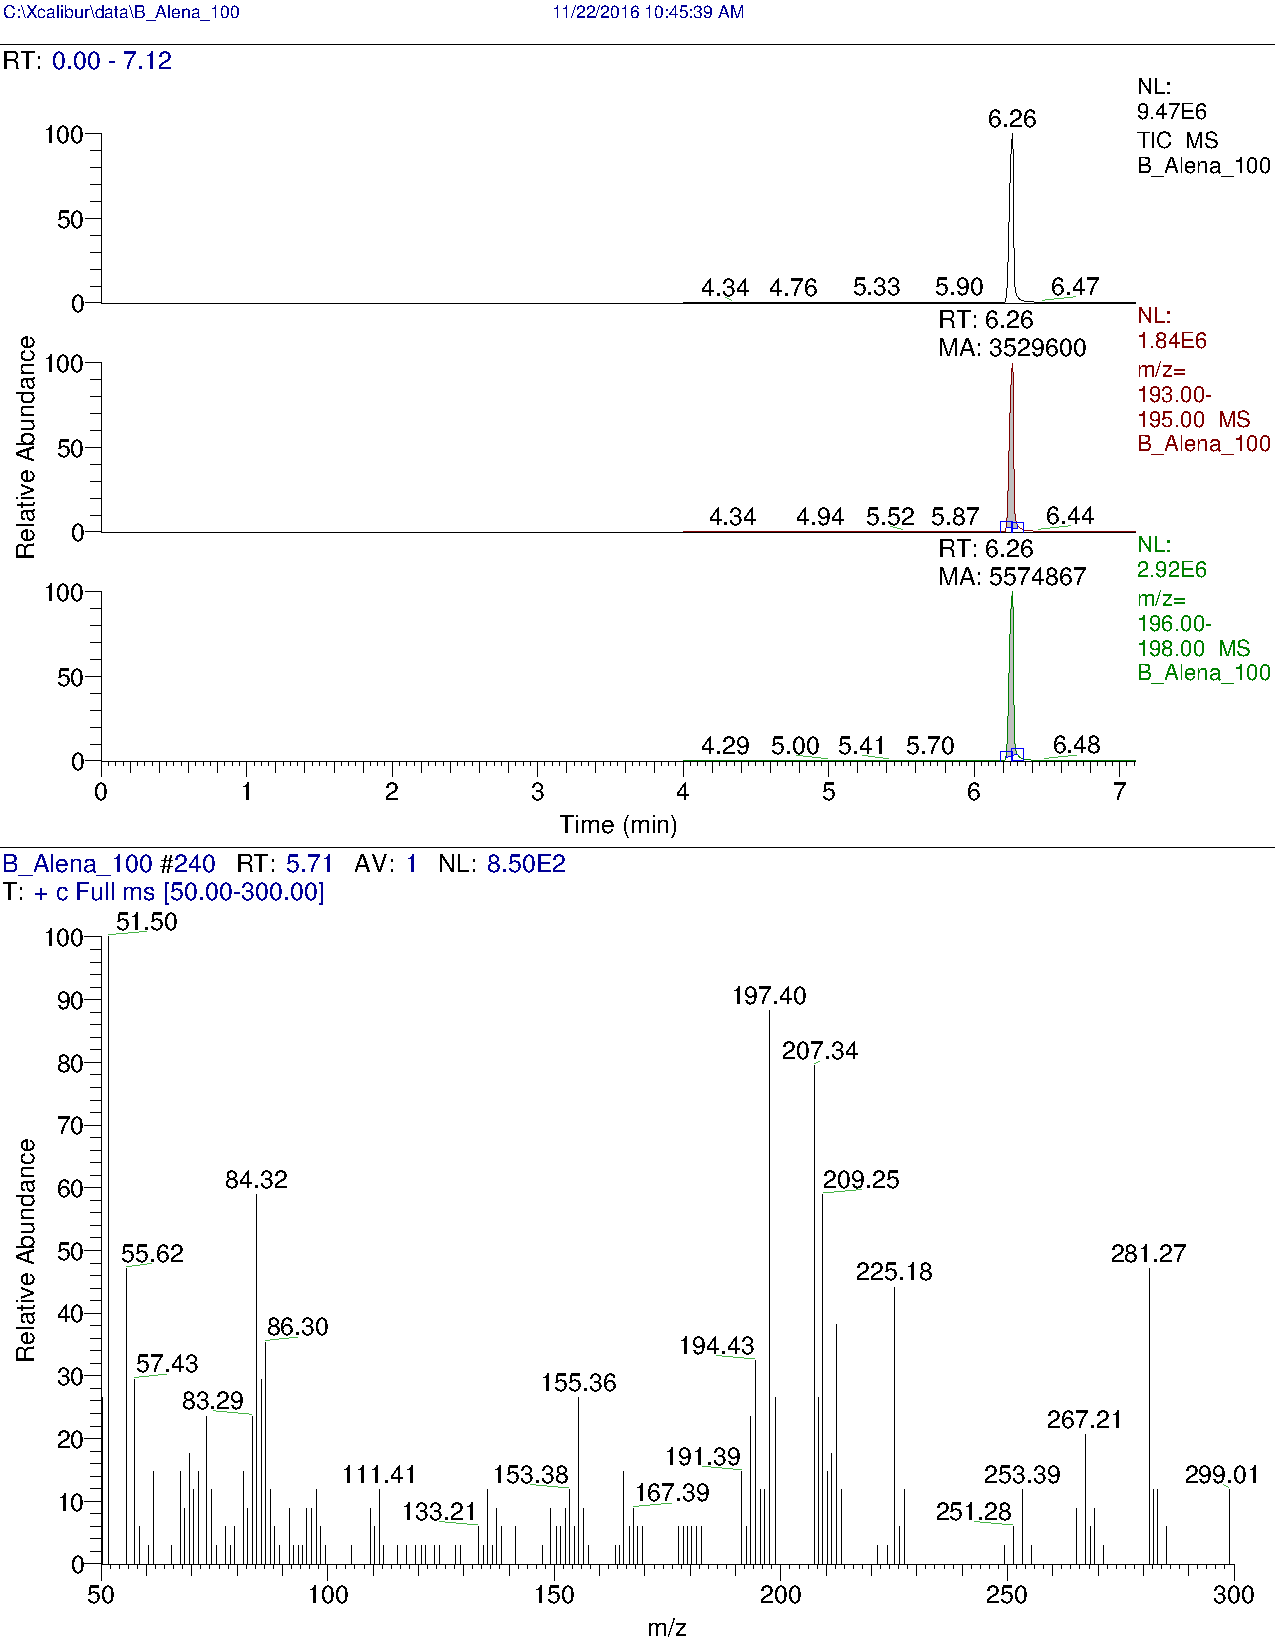
\includepdf[pages=-]{cali100.pdf}
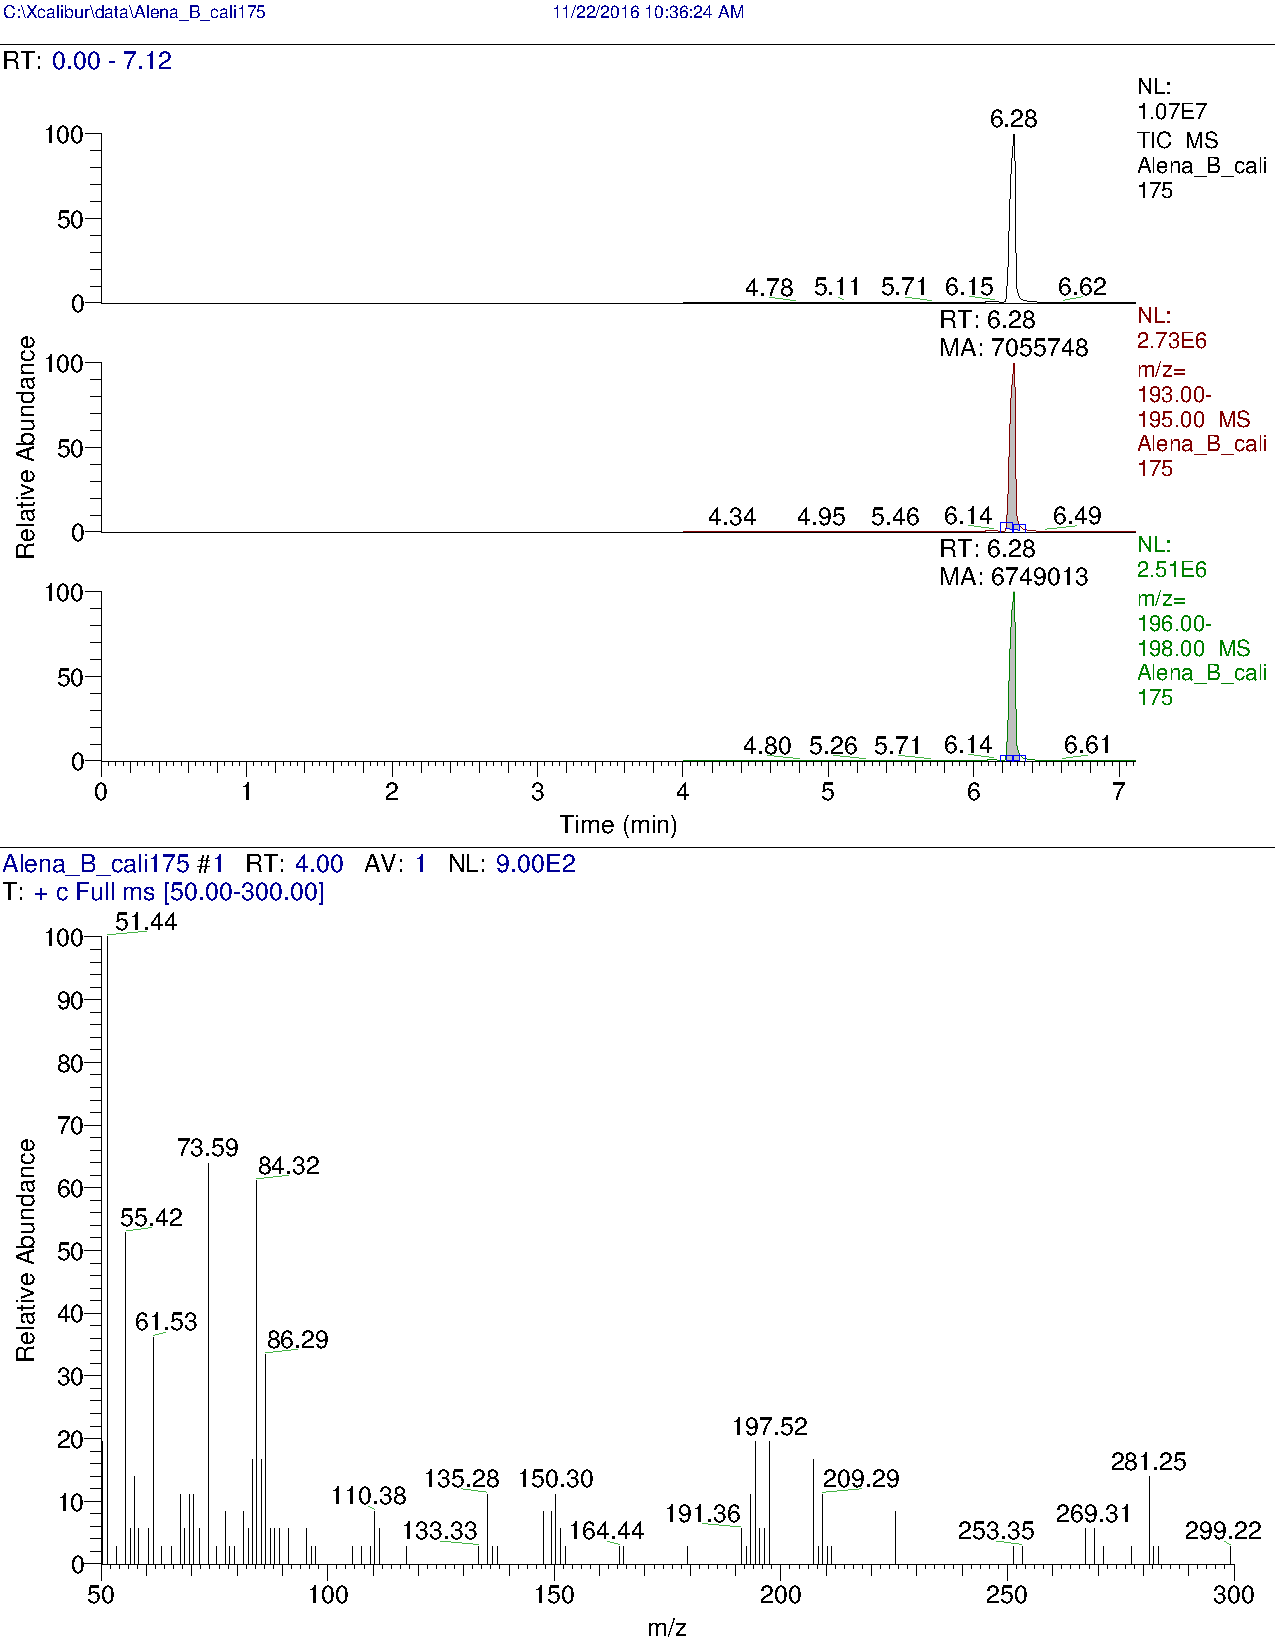
\includepdf[pages=-]{cali175.pdf}
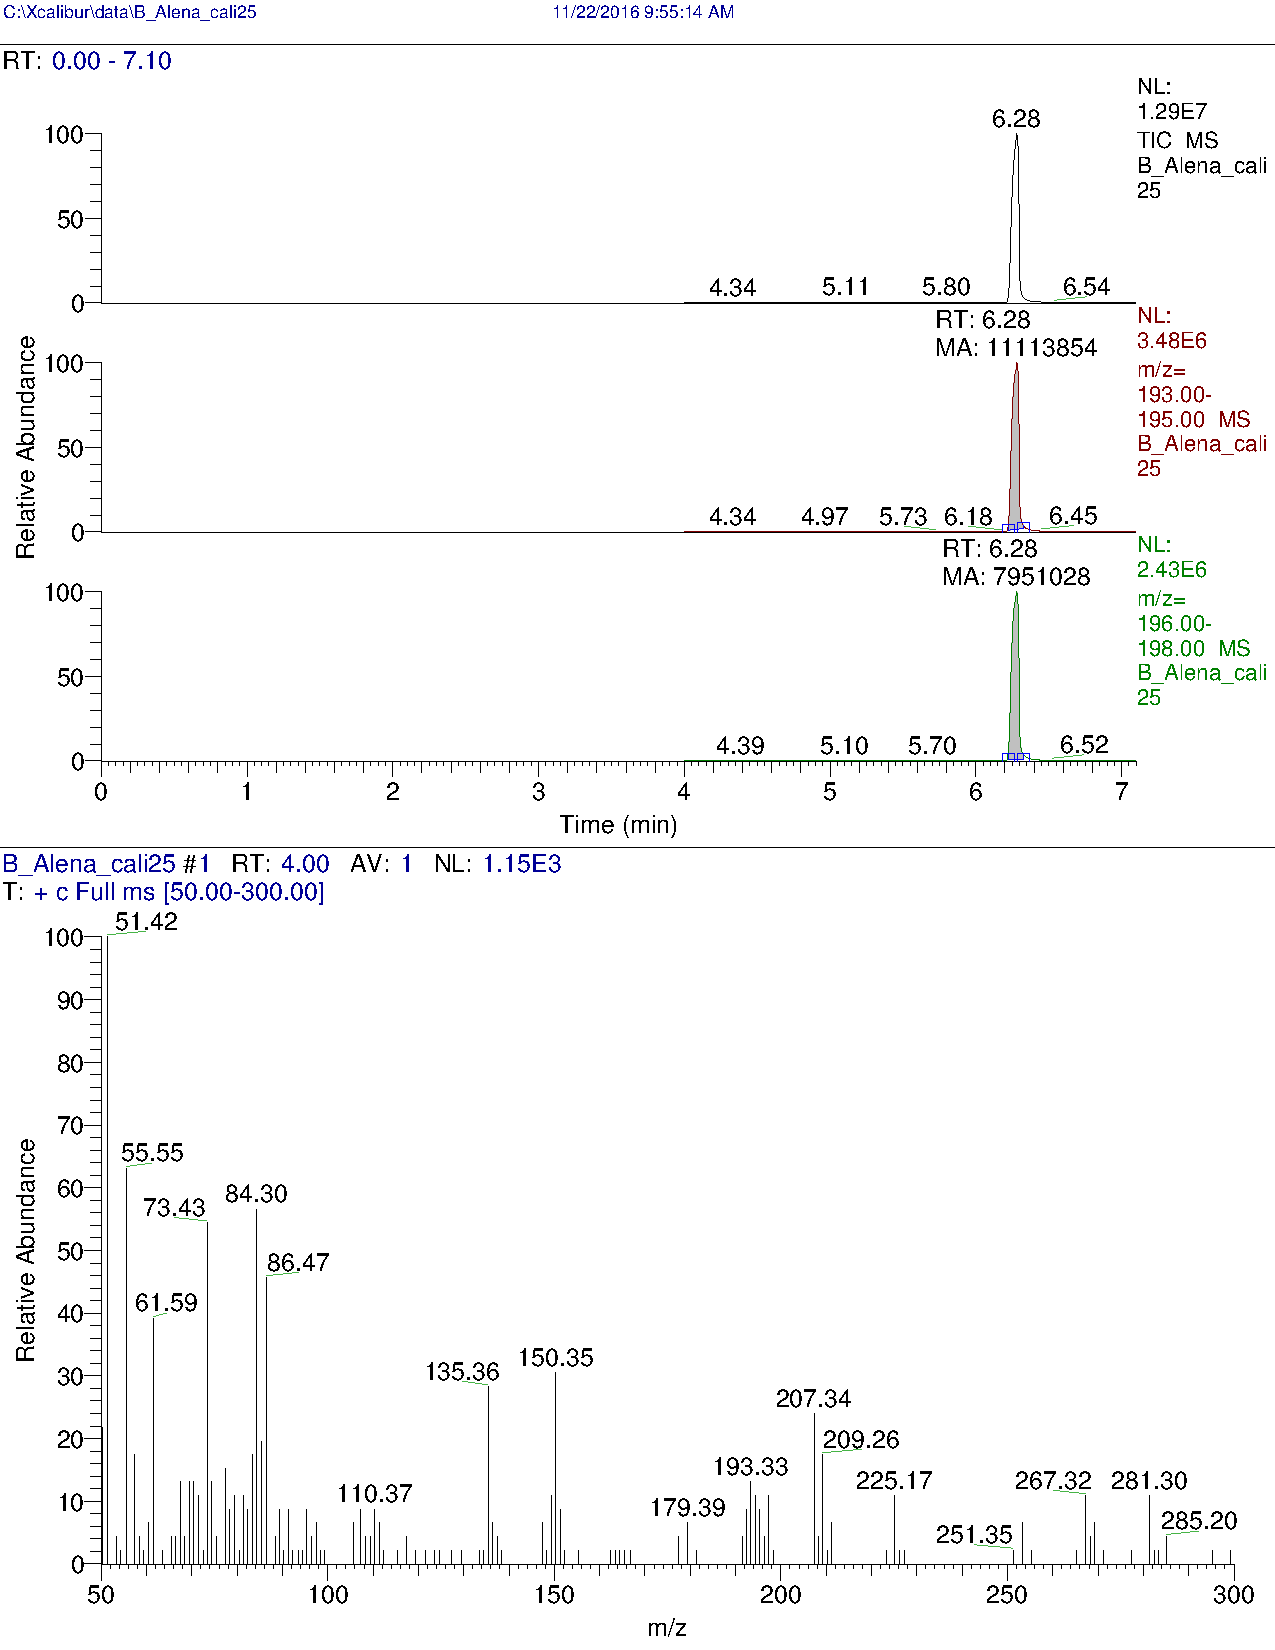
\includepdf[pages=-]{cali250.pdf}
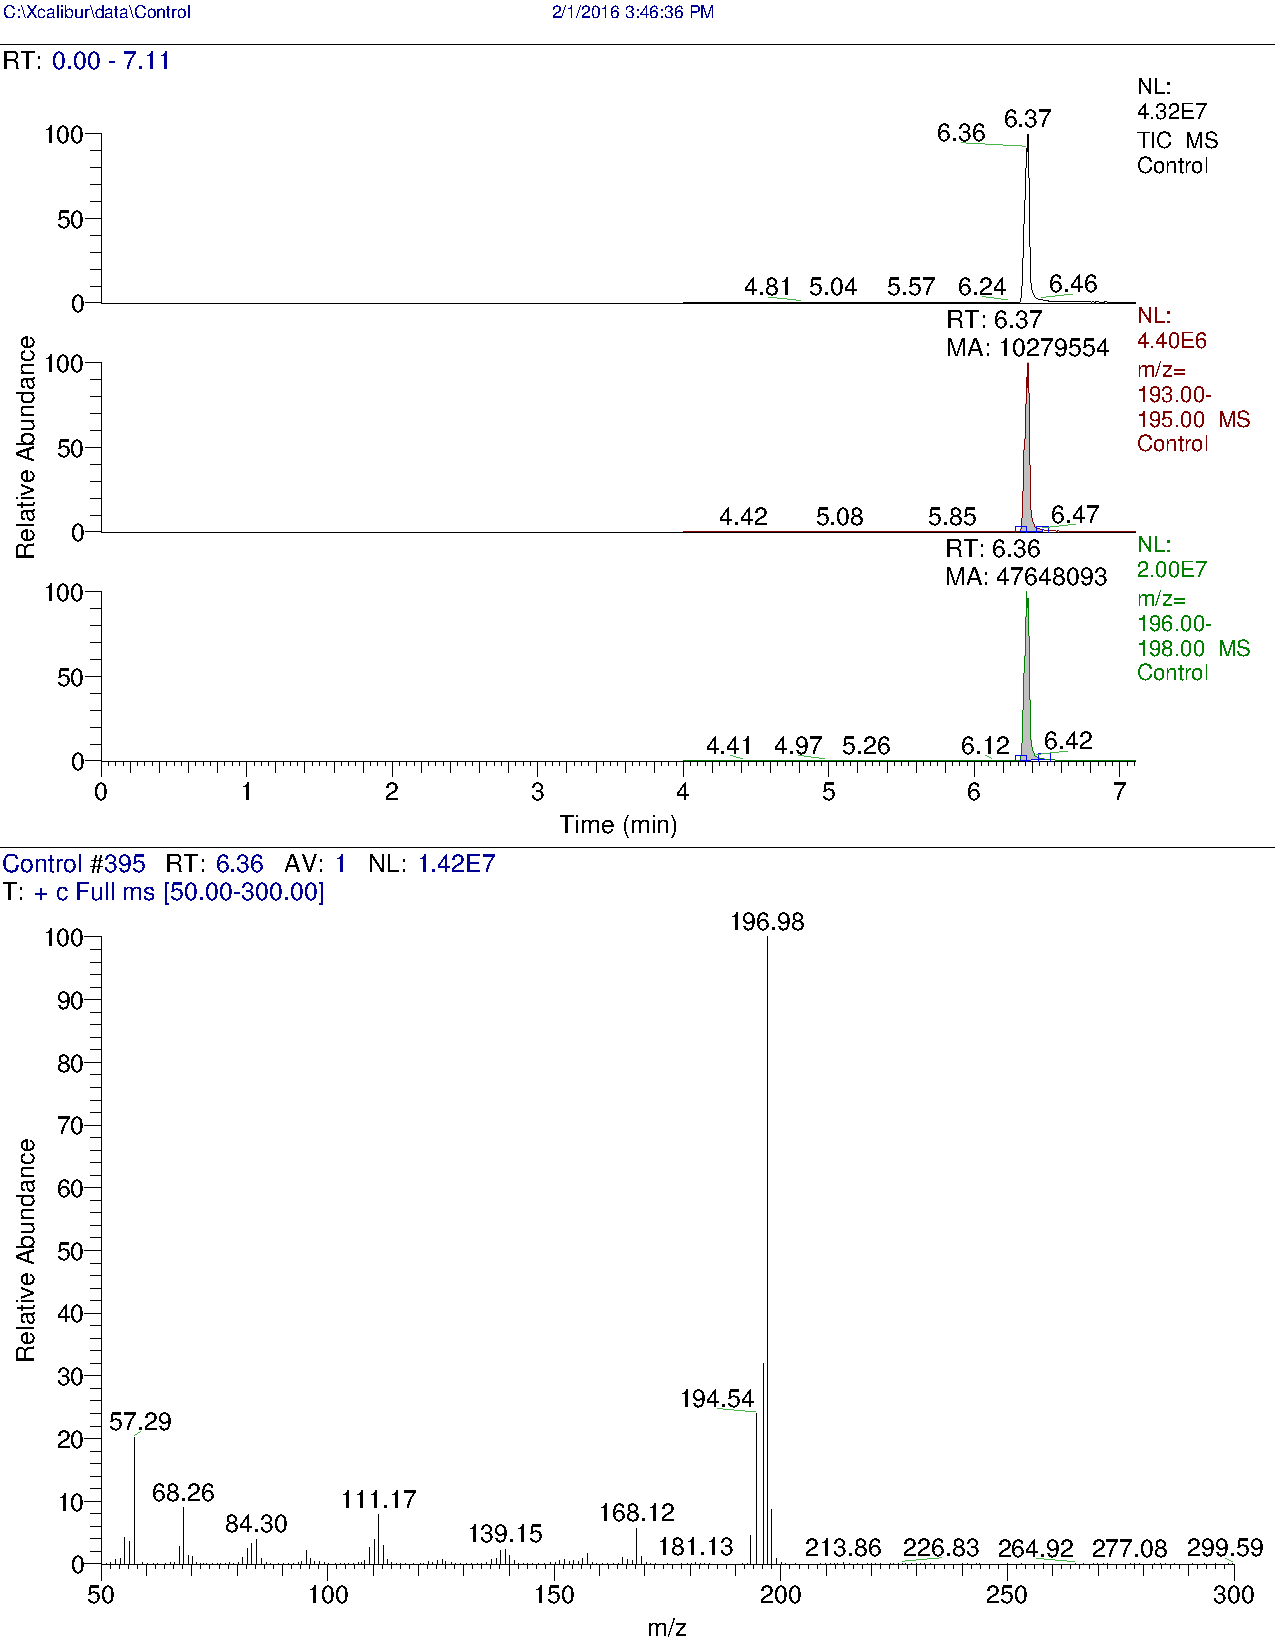
\includepdf[pages=-]{control.pdf} 
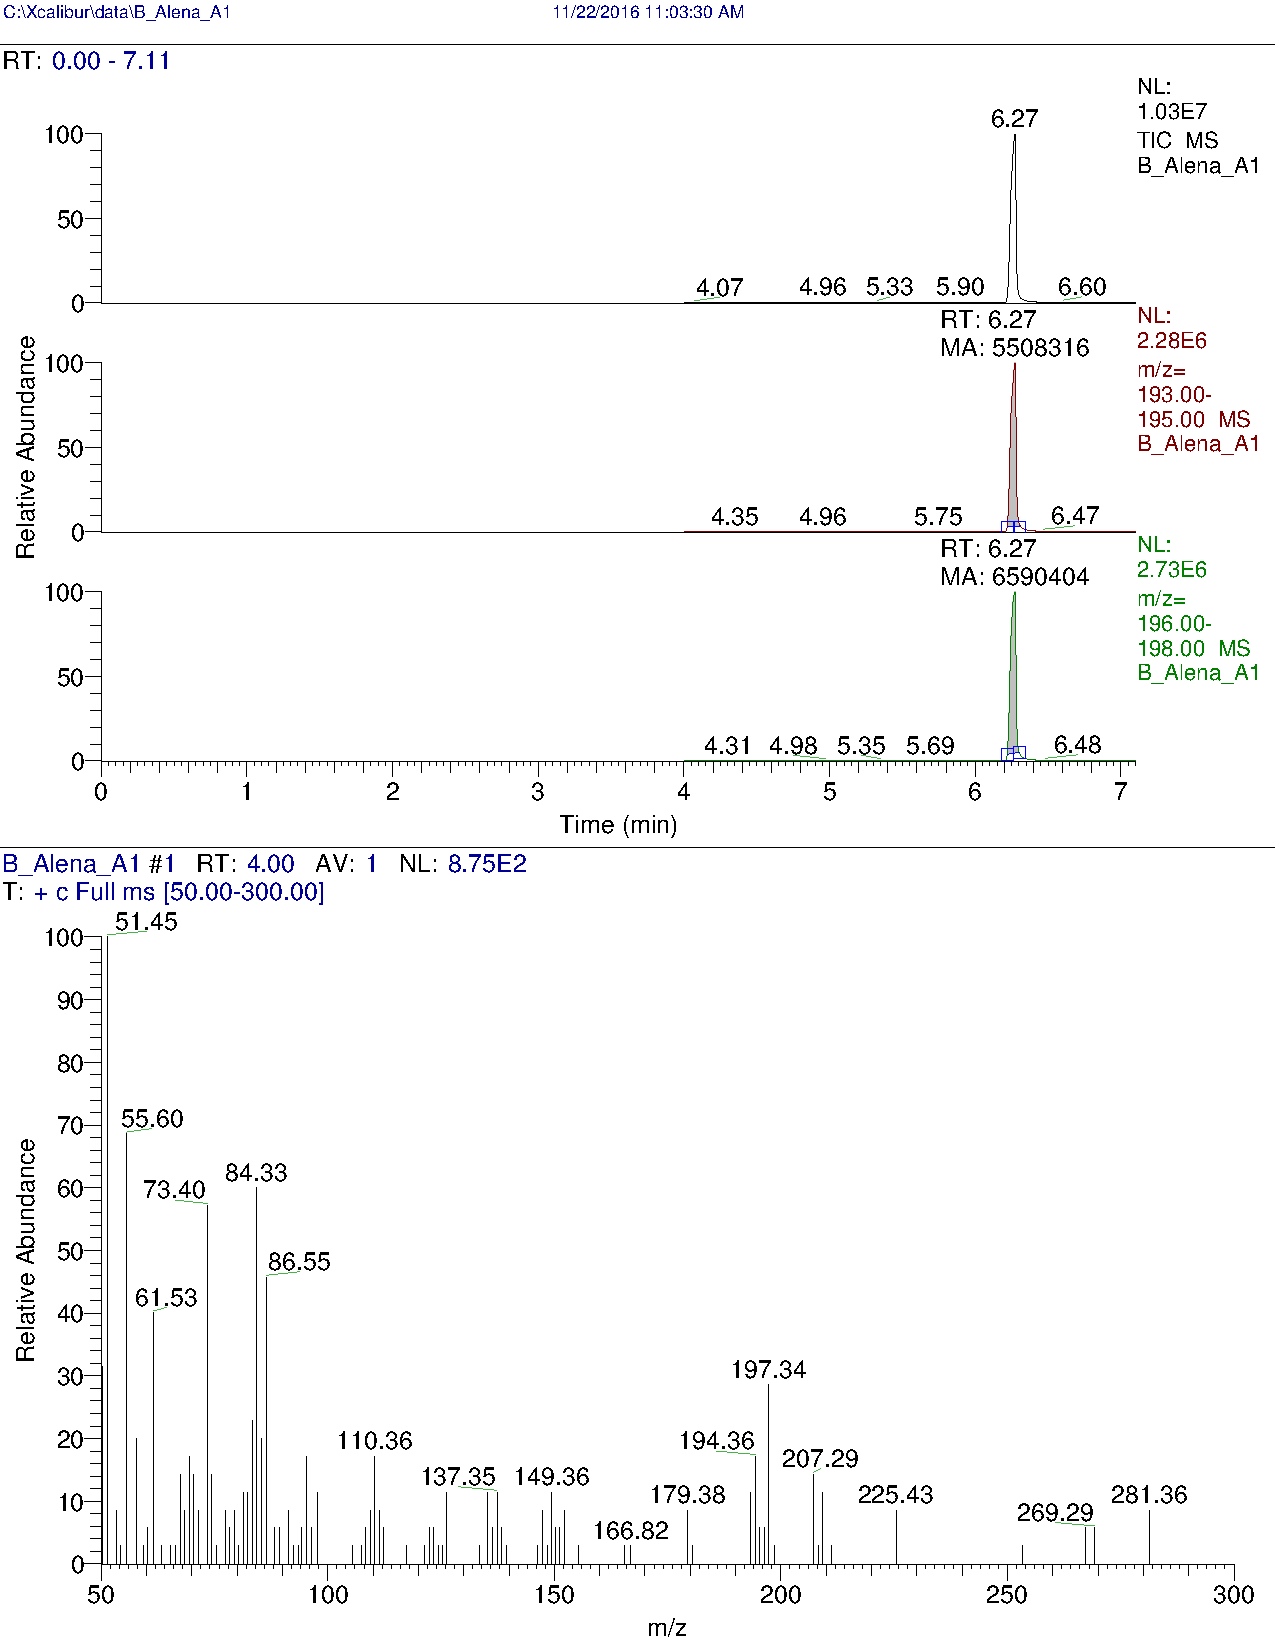
\includepdf[pages=-]{A1.pdf}
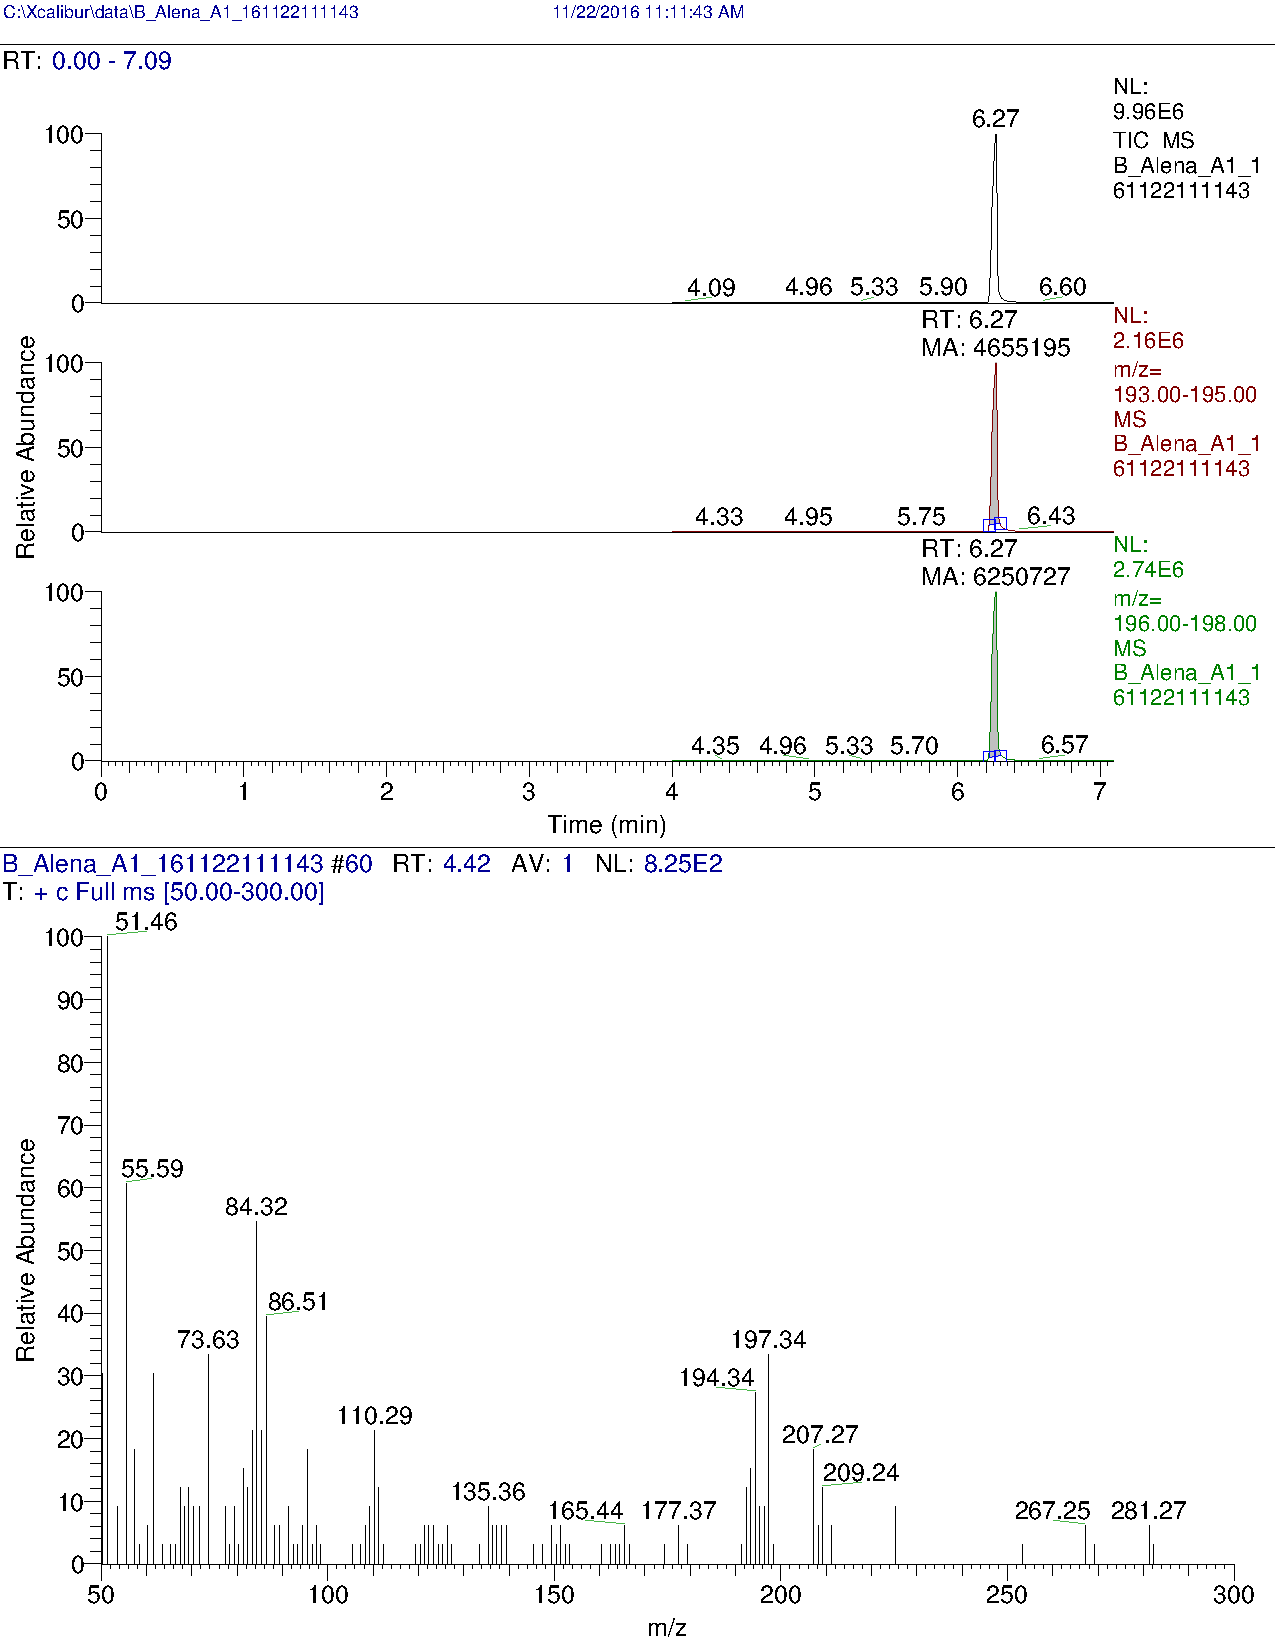
\includepdf[pages=-]{A2.pdf}
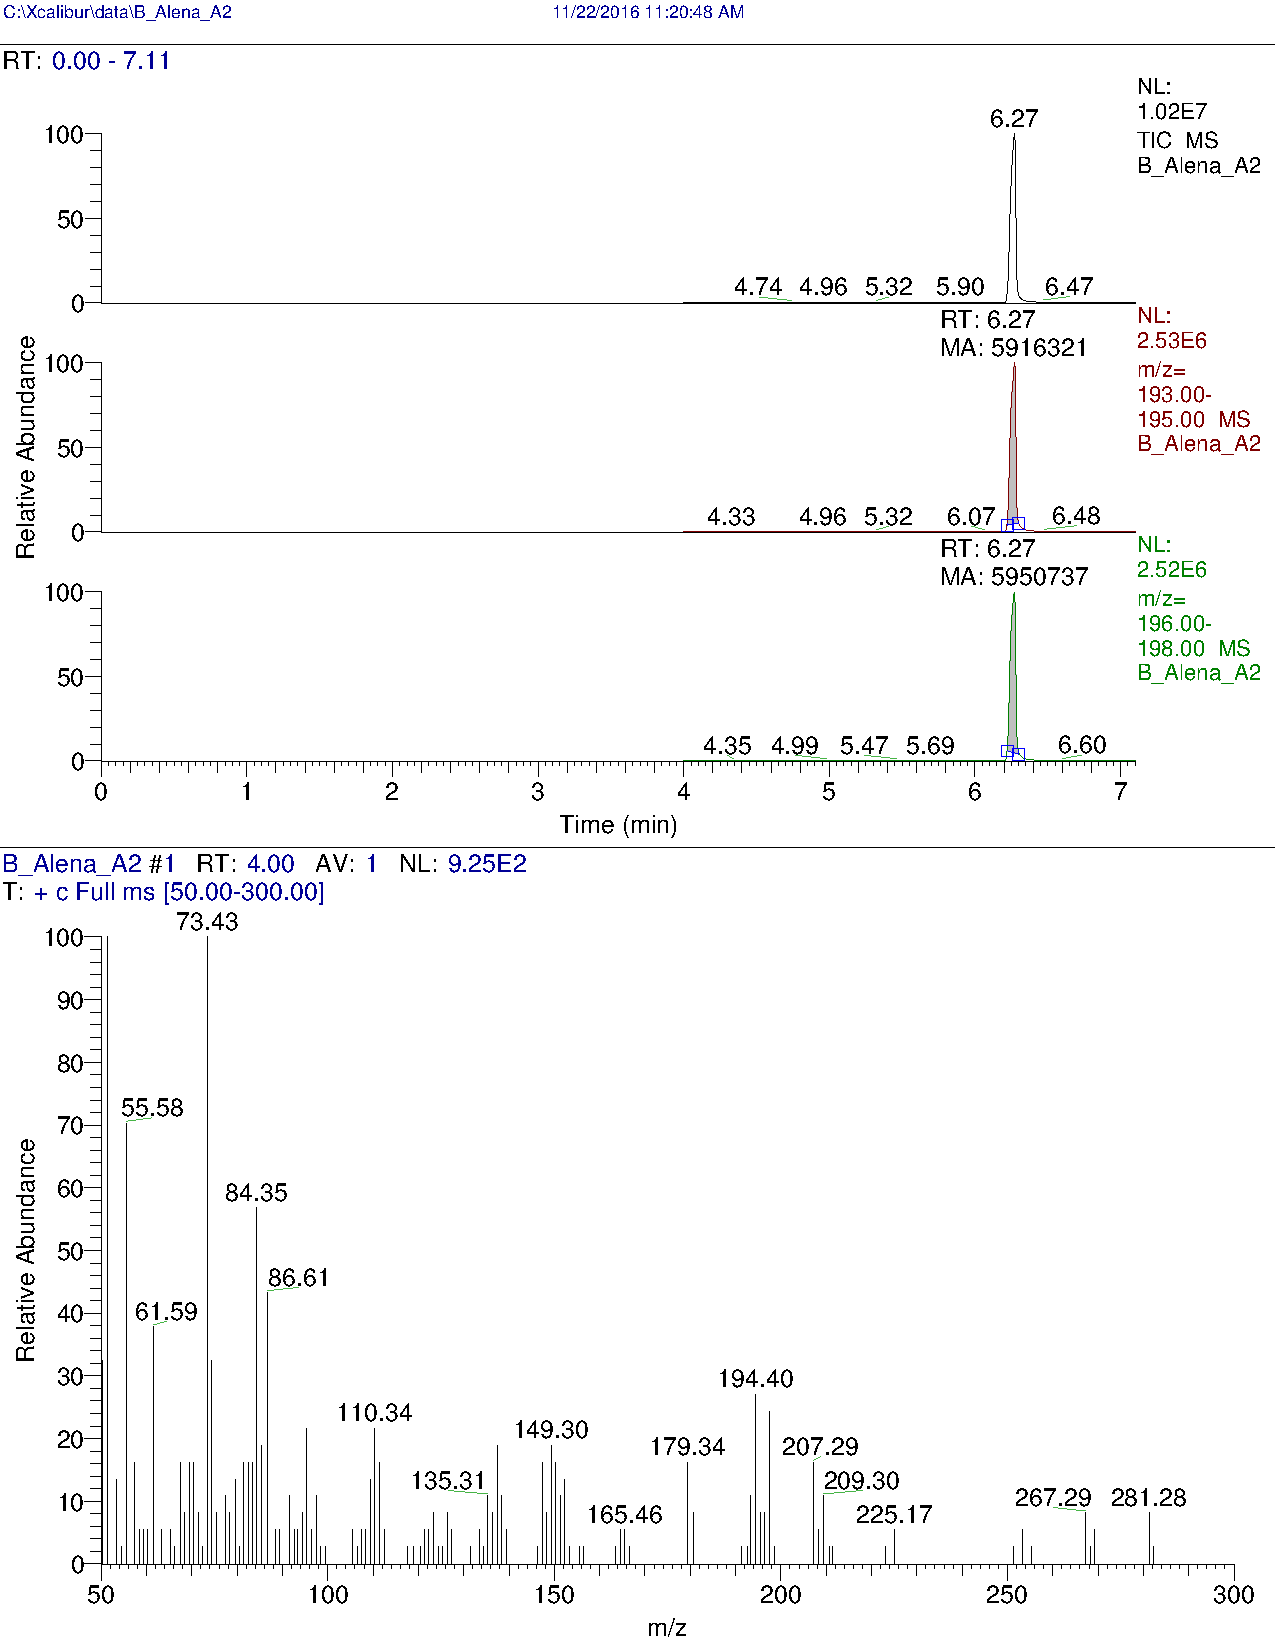
\includepdf[pages=-]{B1.pdf}
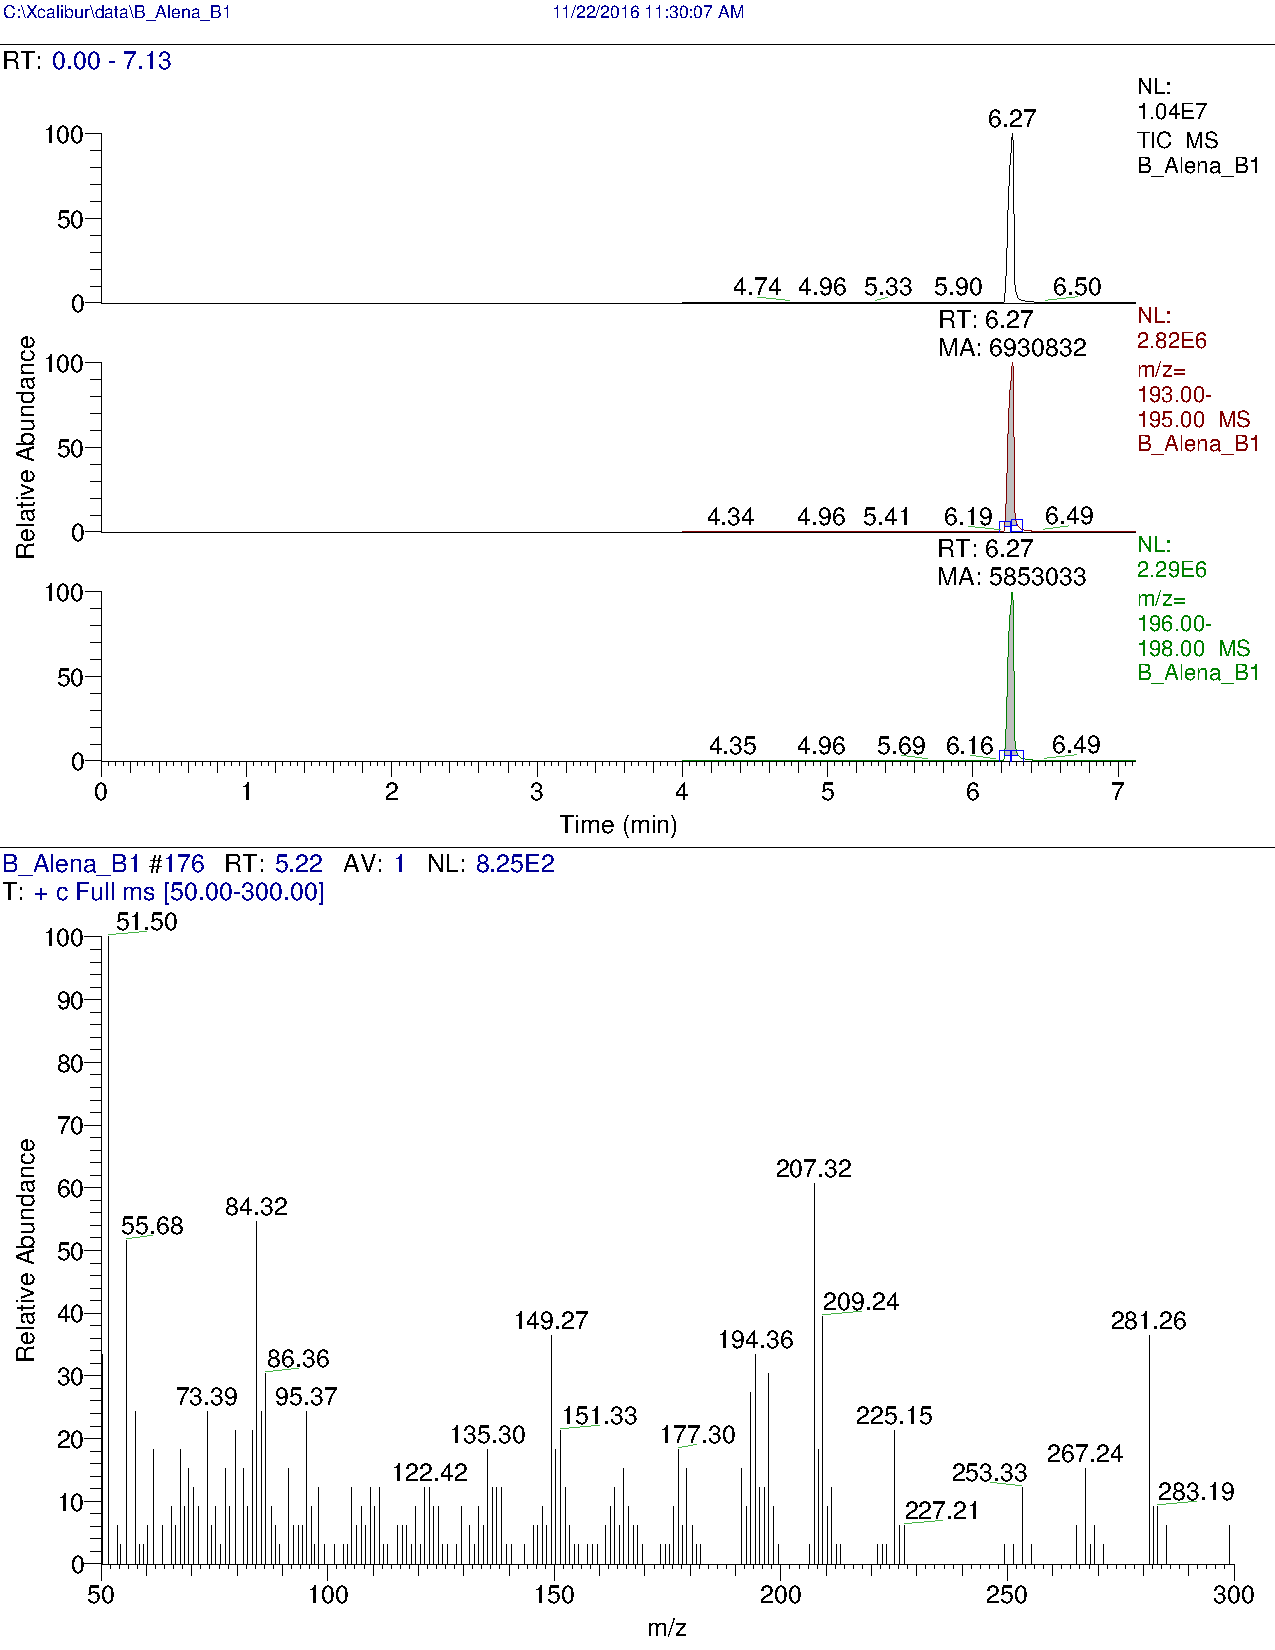
\includepdf[pages=-]{B2.pdf}

Figure \ref{fig:frag} shows a proposed fragmentation pathway for molecular
caffeine.
\begin{center}
    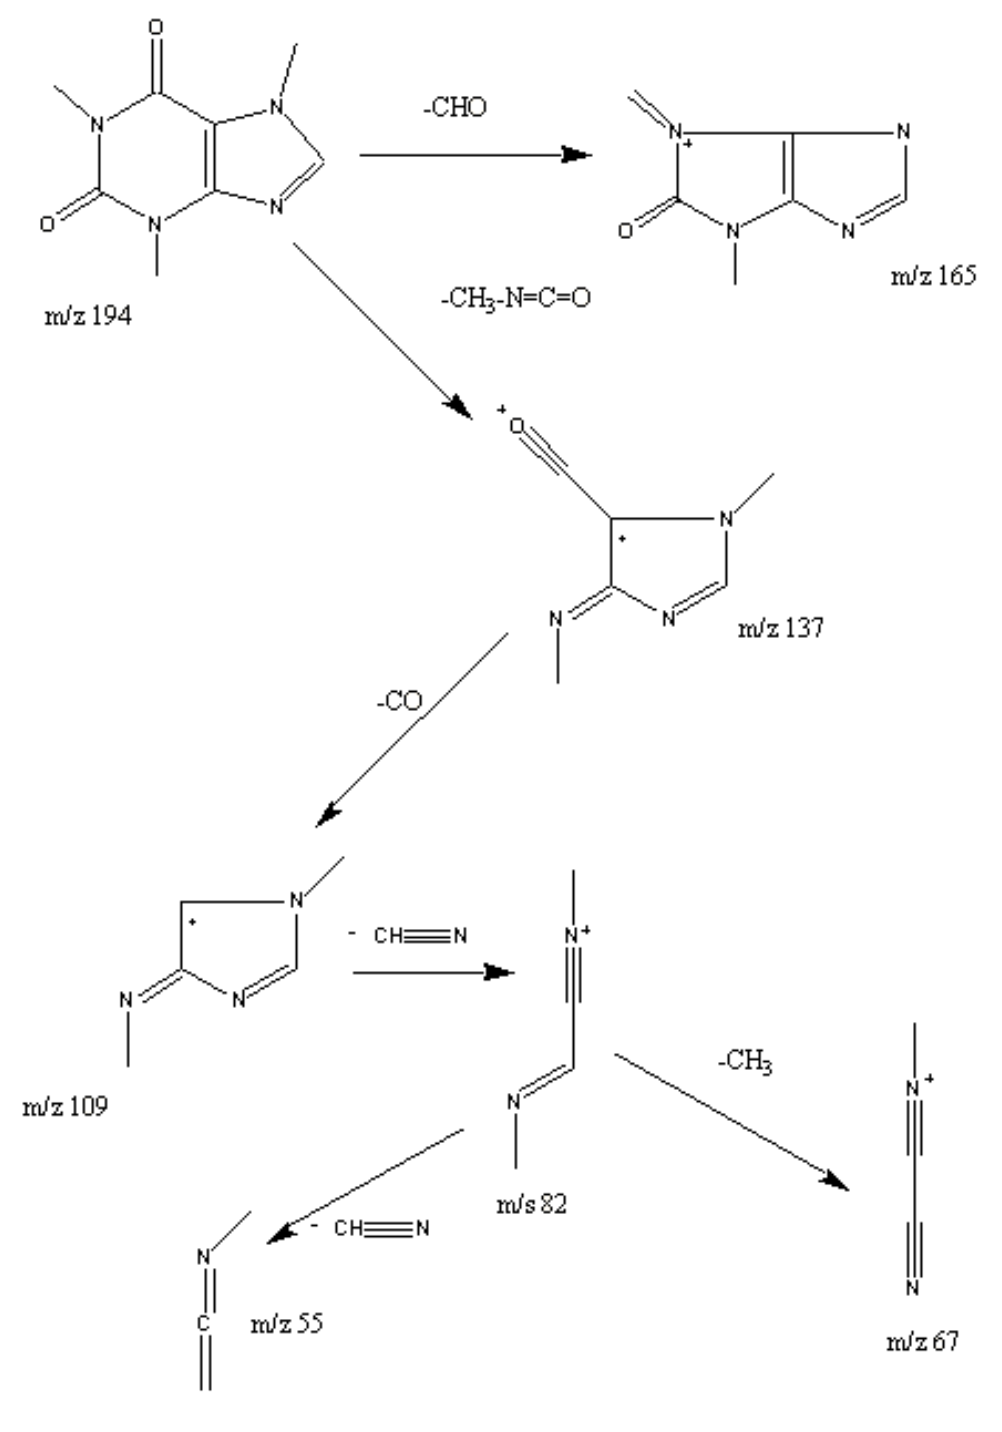
\includegraphics[scale=0.7]{pathway}
    \captionof{figure}{Caffeine molecular ion fragments. \cite{frag}}
    \label{fig:frag}
\end{center}
\newpage

\begin{center}
\subsection*{Sample Calculations for Determining $^{12}$C Caffeine Concentration
in Unknown A}
\vspace{2cm}

    Measured $^{12}$C peak area of run 1: 5508316 \\
    \vspace{0.5cm}
    Measured $^{13}$C peak area of run 1: 6590404 \\
    \begin{equation*}
        \frac{^{12}C}{^{13}C} = 0.8358086
    \end{equation*}
    
    \vspace{1cm}
    fitted line of calibration curve: $f(x) = 0.0049x + 0.0575$ \\ 
    \vspace{1cm}

    $^{12}$C concentration of Unknown A run 1: 158.838 ppm \\
    \vspace{1cm}

    Taking into account dilution factors...
    \vspace{1cm}

    $^{12}$C concentration in original solution: 
    $158.838\ ppm \times 4 = 635.352\ ppm$ \\

    \begin{align*}
        \frac{635.352\ ppm}{33.814} &= 18.790\ mg/fl\ oz \\
        &= 150.32\ mg/8\ fl\ oz
    \end{align*}

    \vspace{1cm}
    Taking into account percent recovery...
    \vspace{1cm}

    $^{12}$C concentration in original solution: 
    $635.352\ ppm \times  1.284 = 815.8\ ppm$ \\

    \begin{align*}
        18.790\ mg/fl\ oz \times 1.284 &= 24.13\ mg/fl\ oz \\
        150.32\ mg/8\ fl\ oz  \times 1.284 &= 193.0\ mg/8\ fl\ oz
    \end{align*}

\end{center}
\end{document} 
